\chapter{Pre-LLM: Storia, Concetti e Task}

\section{Rappresentazioni}

L'approccio classico alla linguistica computazionale è di tipo \fancyglitter{top-down}, occupandosi di codificare il linguaggio naturale in qualcosa di eseguibile da un computer. Tuttavia di recente ha preso sempre più piega l'approccio statistico, \fancyglitter{bottom-up}, sull'analisi qualitativa e quantitativa di fenomeni specifici per effettuare inferenze. 

\subsection{Rappresentazione Vettoriale}

Nel \fancyglitter{text mining} le parole vengono trattate come \textit{token}: sequenze di caratteri prive di significato intrinseco. Un testo è considerato come un insieme di token ciascuno dei quali può comparire con una determinata frequenza. 

\dfn{Vector Space Model (VSM)}{
  Il Vector Space Model (VSM) introdotto da Salton è un modo per rappresentare i testi (fig: \ref{fig:vec}): 
  \begin{enumerate}
    \item Si costruisce un dizionario con tutti i token distinti presenti nel testo associando a ciascuno un indice univoco. 
    \item Si calcolano le frequenze di ciascun token nel testo, ottenendo un vettore numerico che rappresenta il contenuto testuale in forma quantitativa. Se si hanno a disposizione più documenti si ottiene una matrice (generalmente sparsa) in cui:
      \begin{itemize}
        \item Ogni riga rappresenta un documento. 
        \item Ogni colonna rappresenta un token del dizionario.
      \end{itemize}   
  \end{enumerate}
}

\begin{figure}[h]
    \centering
    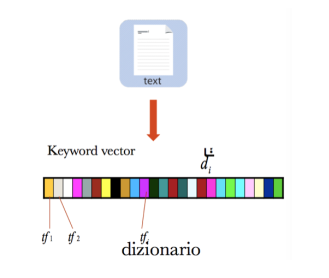
\includegraphics[scale=0.6]{03/vector.png}
    \caption{Rappresentazione testuale tramite VSM.}
    \label{fig:vec}
\end{figure}

\nt{Questa rappresentazione consente di reperire velocemente informazioni anche all'interno di collezioni di miliardi di elementi. Questo è reso possibile grazie all'uso del prodotto scalare tra vettori che permette di calcolare la similarità semantica tra documenti. In questo è molto usata la \fancyglitter{cosine similarity}:
$$\text{similarity} = \cos(\theta) = \frac{A \cdot B}{\|A\| \|B\|} = 
\frac{\sum_{i=1}^{n} A_i B_i}{\sqrt{\sum_{i=1}^{n} (A_i)^2} \sqrt{\sum_{i=1}^{n} (B_i)^2}}
$$
}

\subsection{Metodi Statistici}

I metodi statistici applicati ai documenti si basano principalmente su: 

\begin{itemize}
  \item \fancyglitter{Frequenza dei termini:} rappresenta l'importanza o la rilevanza di una parola all'interno di un documento. Le frequenze assolute non sono sempre efficaci per cui si devono normalizzare. Un approccio utilizzato è il modello \evidence{TF-IDF} che combina due misure:
    \begin{itemize}
      \item TF (Term Frequency): la frequenza di un termine normalizzata rispetto alla lunghezza del documento. 
      \item IDF (Inverse Document Frequency): inversamente proporzionale al numero di documenti in cui il termine appare, calcolata come rapporto logaritmico tra il numero totale dei documenti e il numero di documenti che contengono quel termine. 
        $$TF\!-\!IDF = \frac{n_{i,j}}{|d_j|} \times \log \frac{|D|}{|\{d : i \in d\}|}
$$
    \end{itemize}
  \item \fancyglitter{Co-occorrenza delle parole:} misura la tendenza di due parole comparire insieme all'interno di un determinato contesto (frase, paragrafo, documento, corpus). Si basa sull'assunzione distribuzionale per cui termini semanticamente simili tendono a comparire in contesti simili. Solitamente le co-occorrenze sono rappresentate da una matrice quadrata $|D| X |D|$.
\end{itemize}

\section{Task e Applicazioni Classiche}

\subsection{Tag Clouds}

La prima applicazione sono le tag clouds (fig: \ref{fig:tag}) in cui l'associazione del peso di dominanza a una parola viene espressa attraverso la grandezza della parola stessa in una nuvola di parole. Volendo si può integrare la co-occorrenza mettendo vicine parole simili.
\begin{figure}[h]
    \centering
    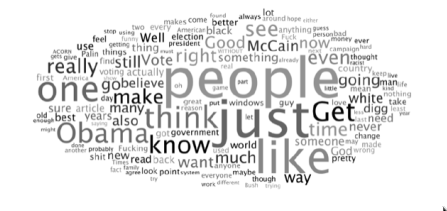
\includegraphics[scale=0.6]{03/tag clouds.png}
    \caption{Esempio di Tag Clouds.}
    \label{fig:tag}
\end{figure}



\subsection{Document Clustering}

Con \fancyglitter{Clustering} (fig: \ref{fig:tag2}) si intende qualsiasi approccio non supervisionato di separazione di documenti in sotto-gruppi più o meno omogenei. Non c'è bisogno di un training set, vengono utilizzate solo frequenze, pesi, co-occorrenze, etc. Esistono due concetti alla base del Clustering:

\begin{itemize}
  \item Non esiste il Clustering perfetto. 
  \item Non esite sempre una misura oggettiva per valutare la bontà di un Clustering.
\end{itemize}

\begin{figure}[h]
    \centering
    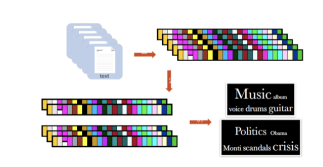
\includegraphics[scale=0.7]{03/clustering.png}
    \caption{Pipeline con clustering e tag clouds.}
    \label{fig:tag2}
\end{figure}

\subsection{Document Classification}

Per la classificazione/categorizzazione (fig: \ref{fig:class}) si vuole ricondurre un testo a una determinata etichetta all'interno di un set di etichette. Per la classificazione è facile effettuare una valutazione perché, avendo già una tassonomia "popolata" con alcune istanze, è possibile fare training con dei testi e poi valutare il modello con altri testi. 

\begin{figure}[h]
    \centering
    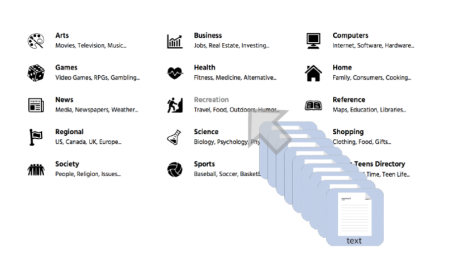
\includegraphics[scale=0.7]{03/classificazione.png}
    \caption{Classificazione di testi su label.}
    \label{fig:class}
\end{figure}

\subsection{Document Segmentation}

Questo task consiste nel separare diverse parti all'interno di un documento cercando di mantenere insieme aree semanticamente coerenti tra loro. L'algoritmo più famoso per svolgere il task è  il \fancyglitter{text tiling}: sull'asse x si ha l'indice del numero della frase, mentre sull'asse y si hanno le parole con la frequenza delle diverse frasi. Il text tiling è una tecnica semplice:

\begin{enumerate}
  \item \fancyglitter{Separazione:} del testo in finestre di lunghezza fissa. 
  \item \fancyglitter{Calcolo della coesione intra-gruppo:} il valore di coesione è semplicemente quanto si usano le stesse parole tra blocchi successivi di frasi (o tokens). 
  \item \fancyglitter{Ricerca:} di parti di testo a bassa coesione circondate da parti di testo ad alta coesione. I picchi più importanti sono quelli verso il basso, ossia i \textit{break-points} (fig: \ref{fig:bp}). 
  \item \fancyglitter{Riadattamento:} delle finestre rispetto al break-point più vicino.
\end{enumerate}

\nt{L'algoritmo è iterativo, quella descritta qui sopra è solo un'iterazione. Al termine delle iterazioni le finestre non hanno più una dimensione prestabilità perché sono state riadattate rispetto ai break-points.}


\begin{figure}[h]
    \centering
    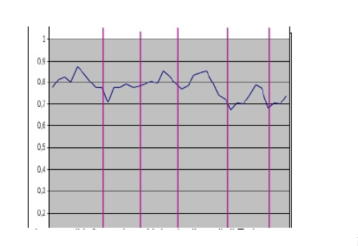
\includegraphics[scale=0.7]{03/breakpoint.png}
    \caption{Break-points nel text tiling.}
    \label{fig:bp}
\end{figure}

\subsection{Document Summarization}

Per ripassare brevemente questo task, esistono due metodi:

\begin{itemize}
  \item \fancyglitter{Estrattivi:} dato un testo o una collezione cercare di dare un valore di \textit{salience} (importanza) alle frasi con l'obiettivo di creare un nuovo documento con quelle frasi. Uno degli algoritmi storici è il \textit{text ranking} che genera un rank delle frasi sulla base della salience. 
  \item \fancyglitter{Astrattivi:} molto più complessi. Sono relativamente recenti e basati su reti neurali avendo in input molti documenti con i loro rispettivi riassunti.
\end{itemize}

\nt{La valutazione di un riassunto è spesso effettuata mediante ROUGE (Recall-Oriented Understudy for Gisting Evaluation): un sistema che mappa gli ngrammi dei riassunti fatti da esseri umani con gli ngrammi dei riassunti generati.}

\subsection{Information Retrieval}

Si basa sul recupero di un documento di interesse sulla base di un seti di keyword (query). Queste ultime possono anche essere collegate a ontologie o metadati. Inizialmente questo task era basato su un modello booleano: si cercava un match diretto. Al giorno d'oggi si effettuano analisi più sofisticate, tenendo in considerazione il contesto e la semantica dei documenti.

\section{Semantica Distribuzionale}

Un'evoluzione del text mining con l'aggiunta dell'uso del linguaggio e dei principi di linguistica. 

\subsection{Introduzione}

\paragraph{Carrellata Storica}

\begin{itemize}
  \item 1954: Harris afferma che le parole che occorrono in contesti simili tendono ad avere significati simili. 
  \item 1957: Firth afferma che una parola è caratterizzata da quelle che la accompagnano. 
  \item 1983: Furnas sostiene che la congiunzione di varie parole permette di specificare più facilmente l'oggetto del discorso. 
  \item 1990: Deerwester: introduce i concetti latenti, con cui afferma che esiste una struttura di base che viene parzialmente oscurata dalla scelta "casuale" delle parole che viene fatta per comporre un discorso. 
  \item 2003: Bley introduce una visione probabilistica secondo cui il tema del documento influenza in modo probabilistico le parole utilizzate nel documento.
  \item 2003: Turney impiega il concetto di \textit{coppie di parole}. Se una certa coppia $(x, y)$ presenta più o meno gli stessi pattern che presenta la coppia $(w, z)$ allora è possibile costruire una sorta di proporzione numerica nel significato delle due coppie. In questo modo si cattura la semantica relazionale.
\end{itemize}

\paragraph{La semantica distribuzionale ha avuto diversi nomi a seconda dei contesti:}

\begin{itemize}
  \item \fancyglitter{Linguistica:} si parla di \textit{Distributional Hypothesis}. 
  \item \fancyglitter{NLP:} \textit{Distributional Semantics}. 
  \item \fancyglitter{Information Retrieval:} \textit{Vector Space Models} o \textit{Latent Semantic Analysis}. 
  \item \fancyglitter{Scienze cognitive:} \textit{Conceptual Space} (i concetti cognitivi sono interpretati attraverso una serie di qualities) o \textit{Graded Categorization} (tutti gli studi che si basano su come il cervello interpreti gli oggetti).
  \item \fancyglitter{Psicometria:} \textit{Hyperspace Analogue to Language}. 
  \item \fancyglitter{Graph Theory:} \textit{Matrici di Adiacenza}.
\end{itemize}

\subsection{Le Matrici}

\qs{}{Perché usare le matrici? Come mai sono state usate solo le matrici? Perché questo approccio funziona bene?}

\paragraph{Risposta:} la rappresentazione vettoriale è un'approssimazione, esattamente come lo è il linguaggio. 

\paragraph{Le matrici sono una via di mezzo:}

\begin{itemize}
  \item \fancyglitter{Rappresentazione simbolica:} propria dei metodi formali di rappresentazione, rende possibile fare inferenze logiche. Nella logica formale i \textit{simboli} sono solo simboli che hanno un potere inferenziale all'interno di una base di conoscenza (KB). 
  \item \fancyglitter{Rappresentazione associazionistica/connessionistica:} teorie legate alle scienze cognitive in cui si pensa che tutto sia connesso con tutto. Il learning consiste nell'apprendere i pesi di tutte le connessioni.
\end{itemize}

\nt{Le matrici facilitano la condivisione della conoscenza in cui il significato diventa una \textit{regione geometrica}.}

\paragraph{Esistono varie tecniche per utilizzare le matrici:}

\begin{itemize}
  \item \fancyglitter{Similarità:} cosine similarity, Jaccard similarity, etc. 
  \item \fancyglitter{Trasformazioni matriciali:} SVD, NNMF, etc. 
  \item \fancyglitter{Clustering:} K-means, EM, etc.
\end{itemize}

\paragraph{Esistono procedure di pre-processing che dovrebbero essere sempre applicate:}

\begin{itemize}
  \item \fancyglitter{Normalizzazione:} procedimento lessicale, sintattico o morfologico, ossia tokenizzazione, lemmatizzazione e stemming. 
  \item \fancyglitter{Denormalizzazione:} arricchimento semantico attuato mediante named entities, semantic roles e associazioni semantiche. Per esempio la WSD può essere considerata una tecnica di denormalizzazione.
\end{itemize}

\paragraph{Nel 2010 Peter Turney distingue tre configurazioni matriciali primarie:}

\begin{itemize}
  \item \fancyglitter{Term-Document Matrix:} considera i documenti espressi come termini. Su ogni riga si ha un documento e su ogni colonna un termine. Questa configurazione viene utilizzata per effettuare il calcolo della similarità, il clustering, la classificazione, la segmentazione, parzialmente il Q\&A, etc.
  \item \fancyglitter{Term-Context Matrix:} è la generalizzazione della Term-Document. Su ogni riga si ha un contesto e su ogni colonna un termine. Un contesto non deve necessariamente essere un documento, ma può essere un paragrafo, una frase, una dipendenza sintattica, etc. 
  \item \fancyglitter{Pair-Pattern Matrix:} la proposta di Turney. Su ogni riga si hanno coppie di parole, mentre su ogni colonna si ha un pattern\footnote{Fortunatamente non un GoF.}. I pattern mettono in relazione tutte le possibili coppie di parole attraverso relazioni. Questa matrice viene usata per calcolare la \textit{relational similarity}, la \textit{pattern similarity}, la \textit{relational clustering} e la \textit{relational search}. 
\end{itemize}

\subsection{Il Ruolo della Similarità}

La similarità è fondamentale, infatti la semantica distribuzionale è anche conosciuta come la semantica della similarità. Negli anni '60, Quine mette in luce il ruolo della similarità nell'apprendimento e nel pensiero poiché consente di categorizzare le cose. Per prevedere le funzionalità di oggetti sconosciuti l'essere umano fa riferimento a oggetti simili di cui conosce l'utilizzo/significato. Nella linguistica computazionale sono definiti vari tipi di similarità:

\begin{itemize}
  \item \fancyglitter{Semantic Similarity:} concetti che hanno quasi lo stesso significato (sinonimia). 
  \item \fancyglitter{Semantic Relatedness:} concetti che condividono proprietà, che hanno affinità semantica. Possono essere meronimi (costituente di qualcosa), antonimi (significato opposto di qualcosa), ma anche sinonimi. Ciò che è semanticamente simile è anche semanticamente relazionato, ma non è vero il contrario. Purtroppo questo tipo di semantica è quasi inutilizzabile perché troppo generica (dice che due concetti sono relazionati ma non il come). 
  \item \fancyglitter{Attributional Semantic:} concetti che condividono attributi (proprietà). In realtà si tratta di Semantic Relatedness. 
  \item \fancyglitter{Taxonomical Similarity:} concetti che condividono più iperonimi (concetti generici rispetto a dei concetti più specifici). 
  \item \fancyglitter{Relational Similarity:} lavora su tuple di concetti. 
  \item \fancyglitter{Semantic Association:} tratta concetti che co-occorrono frequentemente. Molto simile alla relatedness, ma orientata alla corpus analysis. Infatti è possibile avere concetti che non co-occorrono spesso ma che sono comunque relazionati. 
\end{itemize}

\clm{}{}{
  \begin{itemize}
    \item La Distributional Semantic ha come cardine la similarità. 
    \item Tale concetto è fragile perché persone diverse possono attribuire valori diversi alla similarità. 
  \end{itemize}
}

\section{Semantica Documentale}

\dfn{Semantica Documentale}{
  La semantica documentale riguarda tutte le analisi le ricerche effettuate a livello di collezione di documenti.
}

\subsection{Topic Modelling}

\qs{}{Che cos'è un topic modelling?}

\dfn{Topic Modelling}{
  Un topic modelling è un modello statistico o probabilistico che analizza l'uso del linguaggio e individua automaticamente gli argomenti di una collezione di testi.
}

\nt{Il topic modelling è un modello non supervisionato, non necessità di annotazioni manuali.}

Un topic è rappresentato come una lista pesata di parole, non va pensato come un argomento strutturato (passaggio riservato a un'annotazione manuale). I topic vengono estratti con varie tecniche misurando quanto i termini vengono usati negli stessi contesti. È possibile che i topic estratti non siano utili e che siano solo coincidenze.

\dfn{Latent Semantic Analysis (LSA)}{
Prima tecnica di topic modelling, si tratta dell'applicazione di una fattorizzazione matriciale (\textit{Singular Value Decomposition}) che prende in input una matrice, nel nostro caso l'insieme dei vettori del dizionario contenenti le frequenze normalizzate e crea in output tre matrici che approssimano quella di partenza.
}

\clm{}{}{
  \begin{itemize}
    \item La prima matrice è una nuova rappresentazione multidimensionale dei testi ma con nuove features chiamate \fancyglitter{concetti latenti}. 
    \item La seconda matrice è la più particolare: contiene 0 in tutte le celle tranne quelle diagonali in cui contiene i cosiddetti \fancyglitter{Singular Value}. 
    \item La terza matrice è una trasposta delle features latenti.
  \end{itemize}
}

\paragraph{Dettagli di LSA:}

\begin{itemize}
  \item Data la matrice di partenza, con la frequenza delle parole, LSA riconosce le ridondanze.
  \item Nel caso di matrici Term-Document viene catturata l'informazione di co-occorrenza creando nuove features che accorpano tali co-occorrenze, dando vita a concetti latenti in un nuovo spazio vettoriale. 
  \item I concetti latenti possono essere ordinati dal più importante al meno importante, in questo modo si può approssimare in matrici più piccole. 
  \item Viene effettuata un'analisi delle varianze e una riorganizzazione del contenuto sotto forma delle varianze maggiori verso quelle minori. 
  \item SVD applicata a matrici che rappresentano testi ha due vantaggi: 
    \begin{itemize}
      \item Permette di avere molte meno dimensioni. 
      \item Riduce la sparsità dei dati.
    \end{itemize}
\end{itemize}

\ex{LSA}{

  Tratto dagli appunti del prof. Luigi Di Caro.

  Immaginiamo di avere due documenti $d_1$ e $d_2$ all’interno di una grande base documentale. Se si effettua la Cosine Similarity tra $d_1$ e $d_2$ (le celle bianche in figura indicano valori uguali a 0) il risultato sarà zero, ovvero i due documenti saranno identificati come semanticamente dissimili. Ma se i termini in grigio iniziali di $d_1$ e i termini grigi finali di $d_2$ analizzati dal calcolo dell’SVD vengono accorpati all’interno di singoli concetti latenti (poiché co-occorrono all’interno di un contesto indiretto, cioè negli altri documenti che non sono nè $d_1$ nè $d_2$), diventando una nuova dimensione della matrice finale (in arancione, in figura). Su questo nuovo spazio vettoriale, la Cosine Similarity darà un risultato di similarità maggiore di 0, indice di una similarità positiva per quei due documenti.
}

\begin{figure}[h]
    \centering
    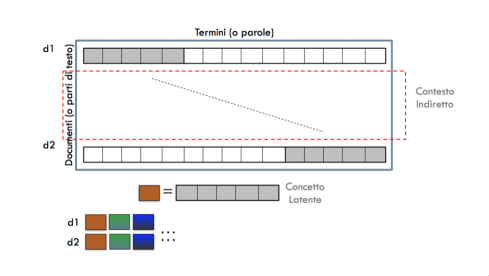
\includegraphics[scale=0.85]{03/ex.png}
    \caption{Contesti indiretti e concetti latenti con SVD.}
\end{figure}

\paragraph{LSA ha alcuni problemi:}

\begin{itemize}
  \item È un modello che non generalizza su documenti non visti: se si aggiungono documenti alla base documentale allora bisogna ricalcore tutto SVD. 
  \item Valori negativi dopo la fattorizzazione sono difficilmente interpretabili. 
\end{itemize}

\paragraph{Dopo la LSA:}

\begin{itemize}
  \item Un'evoluzione naturale si ha nella pLSA, una versione probabilistica. 
  \item Successivamente si passa alla \fancyglitter{Latent Dirichlet Allocation} (LDA) che sfrutta la \textit{statistica Bayesiana}, parte dal presupposto che un documento sia un mix di topics e ogni parola ha una certa probabilità di appartenere a ogni singolo topic. Questa caratteristica ha una duplice funzione, da un insieme di parole:
    \begin{itemize}
      \item È possibile dedurre il topic di appartenenza. 
      \item È possibile dedurre altre parole legate al topic.
    \end{itemize}
\end{itemize}

\subsection{Text Visualization}

Un problema importante per il text mining e la semantica documentale riguarda il come rappresentare uno spazio a $n$ dimensioni (i termini) in uno spazio bidimensionale. 

\dfn{Text Visualization}{
  Area di ricerca che si occupa di studiare come visualizzare il testo in modo tale da riuscire a trasferire un certo contenuto semantico a un utente mediante metodi grafici.
}

\paragraph{Approcci alla text visualization:}

\begin{itemize}
  \item \fancyglitter{Parallel Coordinates:} ogni dimensione viene associata a una coordinata parallela alle altre. Un punto nello spazio multidimensionale diventa una retta che congiunge i valori per quelle dimensioni. Il problema di questo approccio è che se ci sono tanti dati bisogna comprimerli. 

\begin{figure}[h]
    \centering
    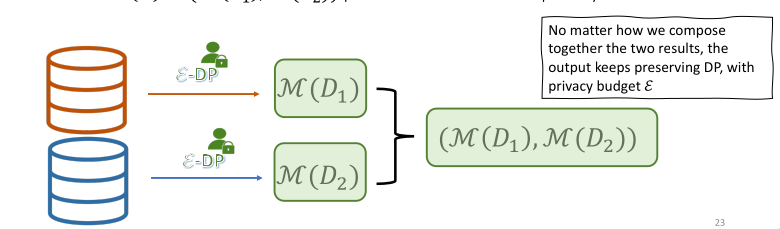
\includegraphics[scale=0.5]{03/pc.png}
    \caption{Parallel Coordinates a 4 dimensioni.}
\end{figure}

\item \fancyglitter{RadViz:} radial visualization. Le dimensioni vengono inserite all'interno di una circonferenza. I punti all'interno sono le istanze mentre la loro posizione deriva dall'attrazione (valore di importanza) delle features poste sulla circonferenza. Il problema è il conflitto gravitazionale tra features differenti che si può annullare a vicenda. 
  \begin{figure}[h]
    \centering
    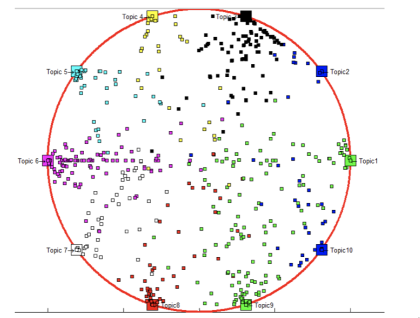
\includegraphics[scale=0.5]{03/rv.png}
    \caption{Visualizzazione con RadViz.}
\end{figure}
\item \fancyglitter{HeatMap:} i dati vengono espressi mediante una matrice e il colore o l'intensità del colore esprime il valore numerico.
\begin{figure}[h]
    \centering
    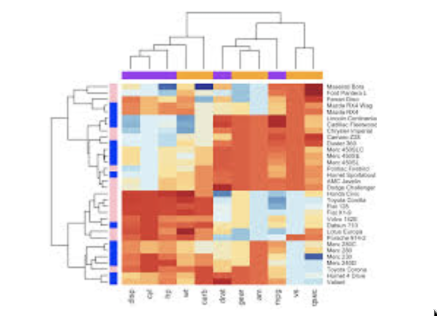
\includegraphics[scale=0.5]{03/hm.png}
    \caption{Visualizzazione con HeatMap.}
\end{figure}
\item \fancyglitter{Correlation Circle:} cerchi in cui sulla circonferenza vengono posti degli elementi e i collegamenti tra questi rappresentano la loro correlazione. 
\begin{figure}[h]
    \centering
    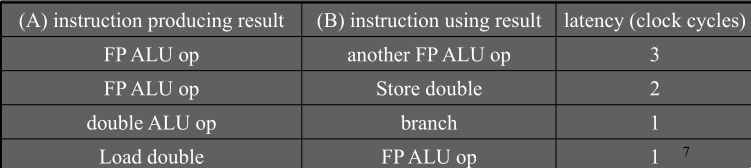
\includegraphics[scale=0.5]{03/cc.png}
    \caption{Visualizzazione con Correlation Circle.}
\end{figure}
\end{itemize}

\section{Ontology Learning e Open Information Extraction}

L'ontology learning è il task che consiste nel costruire un'ontologia con dati non strutturati. 

\subsection{Ontology Learning}

Philipp Cimiano propone una visione dell'ontology learning come reverse engineering: data una conoscenza di un certo dominio, con la sua rappresentazione e la sua codifica si cerca di ritornare alla concettualizzazione di partenza. Questo processo ha due problemi principali:

\begin{itemize}
  \item La conoscenza del mondo non è codificata e quindi non è uguale per tutti. Si possono avere visioni del mondo differenti. 
  \item Non tutto quello che si sa del dominio viene effettivamente utilizzato: si potrebbe conoscere bene un sistema, ma quando lo si va a concettualizzare si pensa al suo utilizzo.
\end{itemize}

\paragraph{Sottospecializzazioni dell'ontology learning:}

\begin{itemize}
  \item \fancyglitter{Ontology Population:} si ha a disposizione un'ontologia già costruita e si vuole analizzare la base testuale per trovare delle istanze da collocare all'interno dei concetti già esistenti dell'ontologia. Si cerca quindi di popolare l'ontologia con nuove istanze. 
  \item \fancyglitter{Ontology Annotation:} data un'ontologia già costruita e una base documentale l'obiettivo è quello di taggare il testo con delle informazioni concettuali come annotazione semantica all'interno di un testo. 
  \item \fancyglitter{Ontology Enrichment:} data un'ontologia già costruita e una base documentale l'obiettivo è dire qualcosa sull'ontologia stessa eventualmente ristrutturandola sia a livello di concetti che di relazioni. 
\end{itemize}

\clm{}{}{
  
  \begin{itemize}
    \item Una rappresentazione più sofisticata è basata su un \textit{thesaurus} (dizionario di sinonimi) come WordNet. 
    \item Man mano che si passa a metodi più sofisticati la difficoltà aumenta.
  \end{itemize}
}

\paragraph{Task dell'ontology learning:}

\begin{itemize}
  \item \fancyglitter{Term Extraction:} trovare nomi per concetti e per le loro relazioni. 
  \item \fancyglitter{Synonim Extraction:} estrazione di paroli con lo stesso significato in determinati contesti. 
  \item \fancyglitter{Concept Extraction:} 
    \begin{itemize}
      \item \evidence{Intensionale:} si cerca di astrarre e rappresentare tutto ciò che un concetto può descrivere. 
      \item \evidence{Estensionale:} si vogliono enumerare tutti gli elementi che descrivono un determinato concetto.
    \end{itemize}
  \item \fancyglitter{Concept Hierarchies Induction:} si cerca di strutturare concetti già noti attraverso una tassonomia. 
  \item \fancyglitter{Relation Extraction:} come Concept, ma per le relazioni. 
  \item \fancyglitter{Population:} spesso fatto attraverso Named-Entity Recognition (NER) o Information Extraction. 
  \item \fancyglitter{Notazione di sussunzione:} meccanismi formali legati al campo della logica matematica che permettono di costruire automaticamente gerarchie.
\end{itemize}

\paragraph{Metodi per soddisfare i tasks:}

\begin{itemize}
  \item NLP: estrazione e uso di informazioni (PoS, NE), pre-processing, regole su alberi di parsing (CKY), informazioni statistiche, risorse lessicali, etc. 
  \item \fancyglitter{Formal Concept Analysis (FCA):} utilizza oggetti (concetti con associate features), attributi e l'incidenza (il fatto che un oggetto abbia o meno un determinato attributo). L'incidenza viene espressa come una matrice chiamata \textit{formal context}. Sulla base del formal context si possono creare operatori per analizzare la matrice per dedurre informazioni. In particolare a ogni elemento si può applicare uno di questi operatori:
    \begin{itemize}
      \item Up: sulle colonne, fornisce gli atributi che un oggetto possiede. 
      \item Down: sulle righe, specifica quali oggetti possidono un determinato attributo.
    \end{itemize}
  \item Machine/Deep learning: addestrare una rete per la costruzione di strutture concettuali e ontologie.
\end{itemize}

\subsection{Open Information Extraction}

L'open information extraction (OIE) nasce dalla necessità di estrarre efficientemente grandi quantità di informazioni da corpora di grandi dimensioni. Queste operazioni son computazionalmente costose, soprattutto se si tratta di miliardi di documenti. Tipicamente si estraggono triple costituite da argomento, espressione verbale e ulteriore argomento. Il problema di questo tipo di estrazione è che si rischia di estrarre molto rumore. Alla fine questo è un approccio data-oriented che permette di effettuare estrazioni \textit{pseudo-semantiche} su un insieme ridotto di dati testuali. Questo approccio è buono per fare Q\&A senza utilizzare un LLM.

\paragraph{Problemi di OIE:}

\begin{itemize}
  \item Non esite un modo rigoroso o unico di estrarre le triple che quindi risultano disallineate in sistemi diversi. 
  \item È difficile valutare e comparare questi sistemi perché non esiste un \textit{gold standard}. 
\end{itemize}

\nt{I sistemi più famosi sono:
\begin{itemize}
  \item ReVerb: basato su vincoli sintattici. 
  \item KrankeN: utilizza WSD. 
  \item ClausIE: non estrae solo triple. 
  \item DefIE: combina parsing e WSD creando un grafo su cui si applicano pesatura degli archi e filtri di rilevanza.
\end{itemize}
}
